\chapter{Anhang 1}
\label{chap:appendix1}

\section{Alternative Figure GCC}
\label{appendix:a1_alternativeGcc}

Figure of \ac{GCC} with filters before the correlation.
\change[]{Better description?}
\begin{figure}[ht]
	\centering
		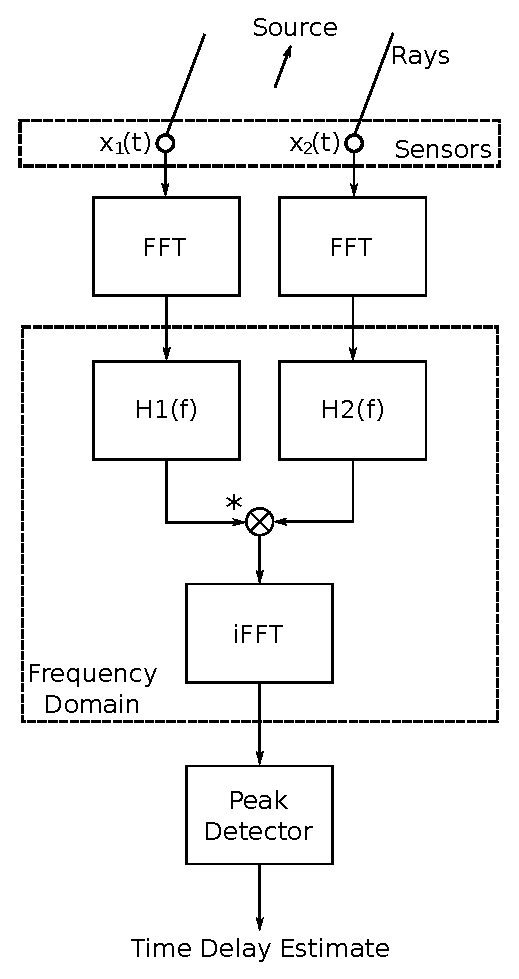
\includegraphics[width=0.35\columnwidth]{figures/GCC}
	\caption{Generalized cross correlation for time delay estimation}
	\label{fig:ap1_GCC}
\end{figure}

\section{Generated Signals for Theory Explanation}
\label{appendix:a1_signals}


Signals used in \cref{sec:02_cc} and \cref{sec:02_gcc} for visualization of the theory.
Both are Hann-windowed sine signals with 3000\si{Hz}, sampled with 44100\si{Hz}.
\lstinline!signal_1! is the same signal as \lstinline!signal_0! but shifted by
10 samples.
\begin{figure}[ht]
	\centering
		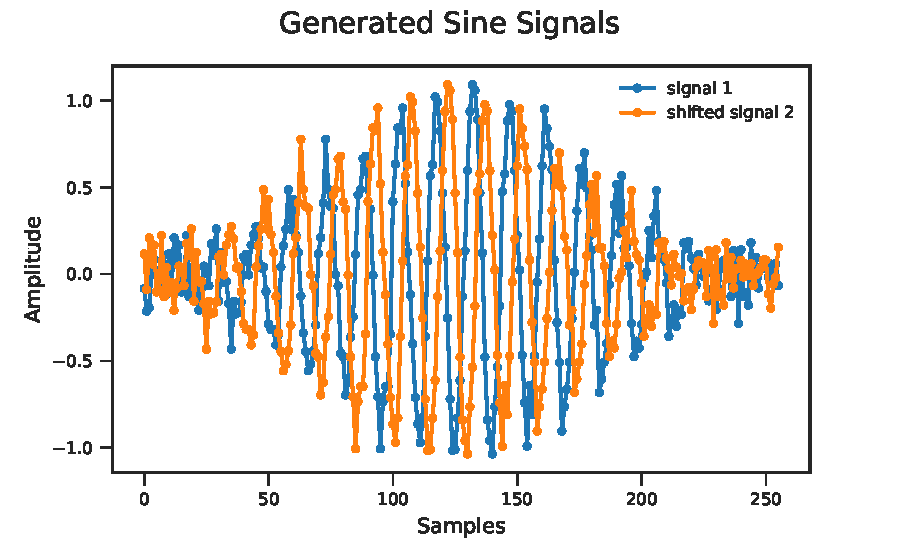
\includegraphics[width=1\columnwidth]{figures/signals_theory}
	\caption{Generated sine signals.}
	\label{fig:ap1_signals}
\end{figure}


